
\documentclass[UTF8]{ctexart}


% PACKAGES FOR TITLES
\usepackage{titlesec}
\usepackage{color}

\usepackage{graphicx}
\graphicspath{ {../../../rc/} }

\usepackage{subfig} % Numbered and caption subfigures using \subfloat
\usepackage{caption} % Coloured captions
\usepackage{transparent}

% STANDARD MATH PACKAGES
\usepackage{amsmath}
\usepackage{amsthm}
\usepackage{bm}
\usepackage[overload]{empheq}  % For braced-style systems of equations

% PACKAGES FOR TABLES
\usepackage{tabularx}
\usepackage{longtable} % tables that can span several pages
\usepackage{colortbl}

% PACKAGES FOR ALGORITHMS (PSEUDO-CODE)
\usepackage{algorithm}
\usepackage{algorithmic}

% PACKAGES FOR ITEMIZE & ENUMERATES 
\usepackage{enumitem}

% PACKAGES FOR REFERENCES & BIBLIOGRAPHY
\usepackage[colorlinks=true,linkcolor=black,anchorcolor=black,citecolor=black,filecolor=black,menucolor=black,runcolor=black,urlcolor=black]{hyperref} % Adds clickable links at references

\usepackage{url}
\usepackage{hyperref}
\usepackage{cleveref}
\usepackage[square, numbers, sort&compress]{natbib} % Square brackets, citing references with numbers, citations sorted by appearance in the text and compressed
\bibliographystyle{plain} % You may use a different style adapted to your field

% OTHER PACKAGES
\usepackage{amsthm,thmtools,xcolor} % Coloured "Theorem"
\usepackage{comment} % Comment part of code
\usepackage{fancyhdr} % Fancy headers and footers
\usepackage{lipsum} % Insert dummy text
\usepackage{tcolorbox} % Create coloured boxes (e.g. the one for the key-words)

% Do not change Configuration_files/config.tex file unless you really know what you are doing. 
% This file ends the configuration procedures (e.g. customizing commands, definition of new commands)
% Configuration package
\usepackage[bottom=2.0cm,top=2.0cm,left=2.0cm,right=2.0cm]{geometry}


% Create color bluePoli (-> manuale grafica coordinata:  https://www.polimi.it/fileadmin/user_upload/il_Politecnico/grafica-coordinata/2015_05_11_46xy_manuale_grafica_coordinata.pdf)
\definecolor{bluePoli}{cmyk}{0.4,0.1,0,0.4}

% Custom theorem environments
\declaretheoremstyle[
  headfont=\color{bluePoli}\normalfont\bfseries,
  bodyfont=\color{black}\normalfont\itshape,
]{colored}

\captionsetup[figure]{labelfont={color=bluePoli}} % Set colour of the captions
\captionsetup[table]{labelfont={color=bluePoli}} % Set colour of the captions
\captionsetup[algorithm]{labelfont={color=bluePoli}} % Set colour of the captions

\theoremstyle{colored}
\newtheorem{theorem}{Theorem}[section]
\newtheorem{proposition}{Proposition}[section]

% Enhances the features of the standard "table" and "tabular" environments.
\newcommand\T{\rule{0pt}{2.6ex}}
\newcommand\B{\rule[-1.2ex]{0pt}{0pt}}

% Algorithm description
\newcounter{algsubstate}
\renewcommand{\thealgsubstate}{\alph{algsubstate}}
\newenvironment{algsubstates}{
    \setcounter{algsubstate}{0}%
    \renewcommand{\STATE}{%
    \stepcounter{algsubstate}%
    \Statex {\small\thealgsubstate:}\space}
    }{}
    
% Custom theorem environment
%\newcolumntype{L}[1]{>{\raggedright\let\newline\\\arraybackslash\hspace{0pt}}m{#1}}
\newcolumntype{C}[1]{>{\centering\let\newline\\\arraybackslash\hspace{0pt}}m{#1}}
%\newcolumntype{R}[1]{>{\raggedleft\let\newline\\\arraybackslash\hspace{0pt}}m{#1}}

% Custom itemize environment
\setlist[itemize,1]{label=$\bullet$}
\setlist[itemize,2]{label=$\circ$}
\setlist[itemize,3]{label=$-$}
\setlist{nosep}

% Create command for background pic
\newcommand\BackgroundPic{% Adding background picture
	\put(237,365){
	    \parbox[b][\paperheight]{\paperwidth}{%
	    \vfill
		\centering
		\transparent{0.4}
		%\includegraphics[width=0.44\paperwidth]{raggiera_polimi.eps}%
		\vfill}
		}
}

% Set indentation
\setlength\parindent{0pt}

% Custom title commands
\titleformat{\section}
{\color{bluePoli}\normalfont\Large\bfseries}
{\color{bluePoli}\thesection.}{1em}{}
\titlespacing*{\section}
{0pt}{3.3ex}{3.3ex}

\titleformat{\subsection}
{\color{bluePoli}\normalfont\large\bfseries}
{\color{bluePoli}\thesubsection.}{1em}{}
\titlespacing*{\subsection}
{0pt}{3.3ex}{3.3ex}

% Custom headers and footers
\pagestyle{fancy}
\fancyhf{}
      
\fancyfoot{}
\fancyfoot[C]{\thepage} % page
\renewcommand{\headrulewidth}{0mm} % headrule width
\renewcommand{\footrulewidth}{0mm} % footrule width

\makeatletter
\patchcmd{\headrule}{\hrule}{\color{black}\hrule}{}{} % headrule
\patchcmd{\footrule}{\hrule}{\color{black}\hrule}{}{} % footrule
\makeatother


\title{Into Modern Graphics Rendering}
\author{wegatron}
\date{2021.11.2}

\begin{document}
\maketitle

\section{现代图形API VS 传统图形API\cite{modernGraphicsAPI}}
传统图形API: OpenGL(ES), D3D\\
现代图形API: Vulkan, Metal, D3D12
\begin{itemize}
\item 渲染管线状态维护
  \\传统的图形API使用隐式、全局的状态管理机制. 缺陷: 1.无法精准的控制管线当前状态; 2.应用程序必须频繁的调用API来设置管线状态和恢复; 3.API还会对每个渲染状态的设置进行校验和二次处理, 比如合并状态统一提交(新型 GPU 会将这些固定管线状态合并成单一硬件状态, 因此需要Driver在运行时为不同的状态组合创建、查找缓存内部的管线状态集合, 这很可能会导致管线卡顿, 同时额外增大了开销).
  \begin{figure}[H]
    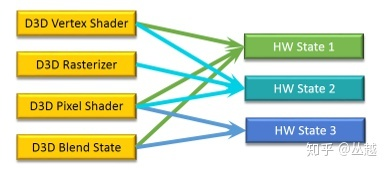
\includegraphics[width=10cm]{render_state_merge.jpg}
    \centering
    \caption{D3D11分散的状态对象设置导致图形硬件切换的额外开销}
    \label{fig:gpu_rendering_pipline_state_merge}
  \end{figure}

  现代图形API使用PipelineState将管道状态提前创建并绑定, 在渲染时, 通过设置不同的 PipelineState, Driver只需要少量的切换开销即可将预先创建的状态绑定到GPU中, 而无需像传统API那样校验每种状态有效性以及动态合并状态, 从而降低了绘制调用开销, 并且可以大幅增加每帧的绘制调用次数.

  \begin{figure}[H]
    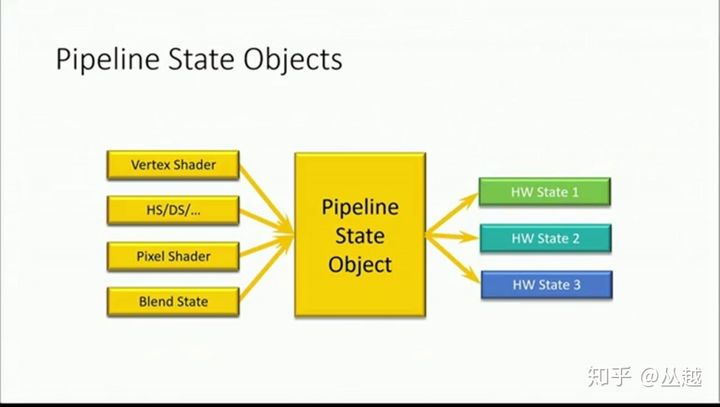
\includegraphics[width=10cm]{pipline_state_object.jpg}
    \centering
    \caption{PipelineState 将管道状态提前创建并绑定}
    \label{fig:graphics_pipeline_state}
  \end{figure}
\item 资源绑定
  \\与渲染管线状态类似, 传统图形API逐个API调用来实现资源的绑定. 而现代图形API通过RootSingature(D3D12) 或者PipelineLayout(Vulkan) 通过Descriptor预先设置好Shader所需要使用的资源布局信息, 包括:Constant、Texture(SRV)、Buffer(UAV)、Sampler 等, 在渲染时Shader通过DescriptorTable或者DescriptorSet用间接寻址方式获取资源, 无需渲染时绑定, 大大降低了资源绑定和校验开销, 从而提高了渲染性能.
  \\Metal 虽然也有 PipelineState, 但并没有提供指定 Shader Resource Layout的机制.
  \begin{figure}[H]
    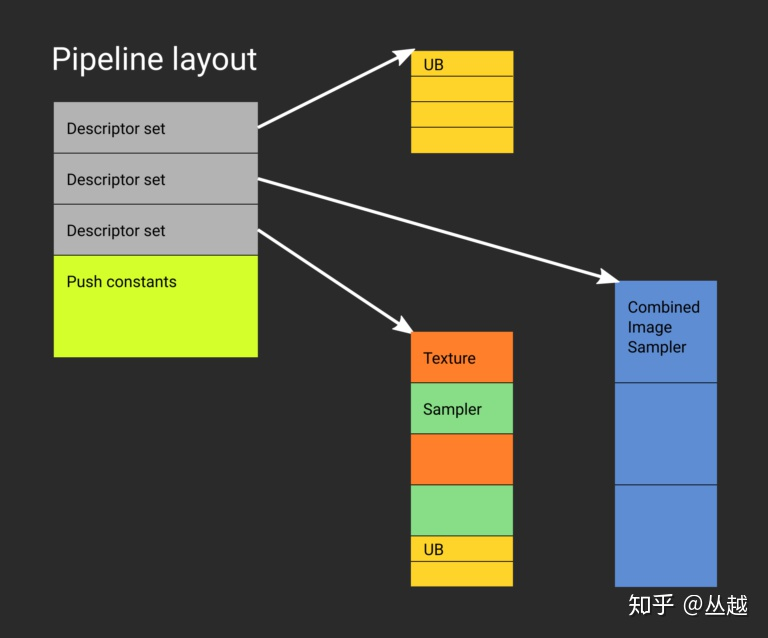
\includegraphics[width=10cm]{data_resource_binding.jpg}
    \centering
    \caption{Vulkan的Pipeline Layout使用DescriptorSet间接引用Shader资源}
    \label{fig:data_resource_binding}
  \end{figure}
\item 显式内存管理
  \\传统的API的内存管理是隐式的, 当创建资源时 Runtime/Driver 内部也同时创建用于这个资源的内存, 这个过程对开发者是透明的, 尽管接口简单, 但带来的问题是很难优化内存分配, 并且容易造成 GPU 内存碎片.
  \\现代API 都提供了 CPU/GPU 堆内存管理接口, 可以通过创建堆, 在堆上分配空间的方式来创建资源, 应用程序可以精准的控制资源堆内存的分配. 比如可以通过资源别名(在同一堆空间中创建不同的资源), 在不同的时段可重复利用同一的设备内存来完成渲染逻辑, 从而更有效的使用有限的 GPU 内存资源.
  \begin{figure}[H]
    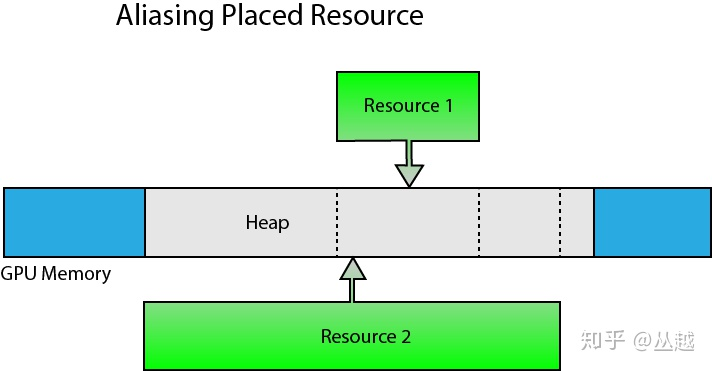
\includegraphics[width=10cm]{gpu_aliasing_placed_resource.jpg}
    \centering
    \caption{在重叠的GPU堆空间中创建不同的资源}
    \label{fig:aliasing_placed_resource}
  \end{figure}
\item 状态的跟踪和同步
  \\传统 API 在 Driver 内部维护跟踪状态, 自动管理资源及调度, 以及进行运行时的校验. Driver 还要负责 CPU 与 GPU 的同步. 典型的例子: 动态更新 GPU Buffer 数据, 如果此时 GPU 正在使用这个 Buffer, 则 Map/Lock 之后 API返回的是 Runtime/Driver 内部动态创建的新内存地址, 以更新新数据, 当 GPU 使用完旧内存后, 再使用新数据. 另外, API 的提示标记并不能保证 Driver 一定按照预想的方式执行, Driver 会根据自身当前的状态来决定, 比如上述情况, 即使在 Map 时指定了 Discard, 也不能完全保证运行时 CPU 和 GPU 是完全异步的.
  \\现代 API 通过使用资源屏障 (Resource Barrier) 来要求应用层明确控制资源的状态迁移, 通过Fence对象和WaitFence函数完成CPU和GPU的同步. 整个过程完全由应用程序来控制, 这样应用程序可以根据需要, 更加精准的控制同步时机.
\item 并行渲染
  \\现代 API 都增加了 Command List 或 Command Buffer 记录渲染指令, 再通过 Queue 提交到 GPU 中, 而每个 Command List/Buffer 都可以在不同的线程中单独填充, 这意味着可以并行录制渲染指令, 充分发挥了现代 CPU 多核的并行能力. 甚至还可以创建多个异步计算或者上传数据的 Command Queue, 利  用 GPU 的并行机制实现渲染和计算、上传数据的并行.
\item shader code
  \\Shader Code预编译机制
\item 附加模块支持
  \begin{itemize}
  \item RayTracying
  \item ML: Vulkan ML, Metal Performance Shader
  \end{itemize}
\end{itemize}

\section{基于现代图形 API 开发的挑战\cite{modernGraphicsAPI}}
要在现代 API 基础上实现更好的性能, 需要更多更复杂的图形管线管理开发工作. 由于是显式的, 更接近图形硬件的设计, 现代 API 的驱动不再负责传统 API Driver 复杂的内部逻辑, 但这些工作并不是自动消失, 而是转移到应用层, 由开发者负责. 传统 API 上和现代 API 上图形管线管理开发工作量的比较:
\begin{figure}[H]
  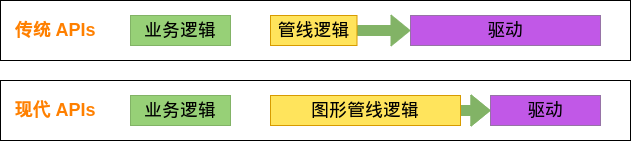
\includegraphics[width=10cm]{graphics_works.png}
  \centering
  \caption{基于传统API和现代API上图形管线管理代码量的比较}
  \label{fig:works_comparation}
\end{figure}

这些工作量包括:
\begin{itemize}
\item 重新设计图形 API 抽象接口.
  \\通过PipelineState对象来维护渲染管线状态, Command List录制图形指令, 实现并行渲染. 资源屏障等, 来进行同步.

\item 堆内存管理.
  \\包括 GPU 和 CPU 内存, 精细控制内存预算和跟踪内存分配和使用, 甚至还要根据不同使用场景来定制内存管理策略. 比如根据 GPU 是否只读、CPU 是否只读、CPU/GPU 的写入频率等, 不同的情况需要对应不同的内存管理策略, 充分利用 GPU 的 Copy/Upload/Transfer 硬件引擎完成数据传输, 才能实现最佳的性能.

\item 描述符(Descriptor)管理
  \\在传统 API 上绑定 Shader 资源只需要简单调用形如 SetTexture/SetConstant/SetSampler 之类的接口即可, 而在现代 API 中, 通过 Shader 所需要使用的资源布局信息是预置的(前文所述), 渲染时需要通过 Descriptor 来间接寻址资源, 由于 Descriptor 也是一种 API(GPU 硬件) 资源, 一般来说 GPU 可见的 Descriptor 是有限的(硬件相关限制), 渲染时需要对有限的 GPU Descriptor 使用有效的管理方式加以重用, 才能完成复杂的渲染逻辑. 另外由于并行渲染的存在, Descriptor 的分配和释放还要考虑到线程同步, 如何在并行中减少线程同步所带来的开销也是需要仔细考虑的问题, 这进一步增加了管理复杂度.

\item 渲染帧管理
  \\为了最大化并行 CPU/GPU, Swapchain 通常需要创建多个back Buffer, 这样 GPU 绘制当前帧(或者上一帧), CPU 可以并行填充绘制下一帧的命令, 在开始录制每个 Frame 的渲染指令时, 可以通过这一帧上一次绘制的 GPU Fence 查询 GPU 是否完成上一次渲染, 如果完成则开始录制逻辑, 否则等待. 要达到这样的结果, 每个 Frame 需要有自己的 CommandList 和相关的 GPU 资源, 这就需要实现渲染帧逻辑, 还需要在提交到 GPU 渲染时对 Frame 进行调度管理.
  \begin{figure}[H]
    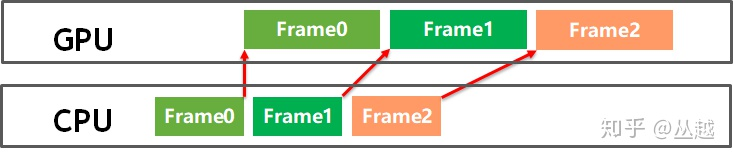
\includegraphics[width=10cm]{frame_management.jpg}
    \centering
    \caption{并行渲染}
    \label{fig:parallel_rendering}
  \end{figure}

\item API 对象的生命周期控制
  \\要保证 API 渲染、计算管线中在使用对象的过程中不能释放对象. 比如上层逻辑在 Frame2 中释放某个对象, 但这个对象还在 Frame1 中被使用, 则此时不能执行真正的释放, 需要通过 GPU Fence 事件通知或者轮询方式等到 Frame1 执行完成才能释放.

\item 并行提交绘制指令
  \\现代 API 的 Command List 都是 Thread Free 的, 所以可以实现多个线程并行填充绘制、计算指令, 以达到并行提交渲染工作的的目的. 可利用Task/Job System来实现.
\end{itemize}

\section{基于现代图形 API 的渲染管线设计\cite{modernGraphicsAPI}}
GPU 并行架构
利用并行提交特性, 渲染管线可设计为多线程结构, 可根据当前 CPU 硬件线程数量动态决定 CommandList/Buffer 的数量, 这样在架构上也是可缩放的。

另外, 现代GPU其内部都会有多个专用于不同功能的GPU硬件, 一般可以抽象为图形(3D)、计算(Compute)、Copy(Transfer)三种, 这三者在 GPU 内部可并行执行, 如下图所示:

\begin{figure}[H]
  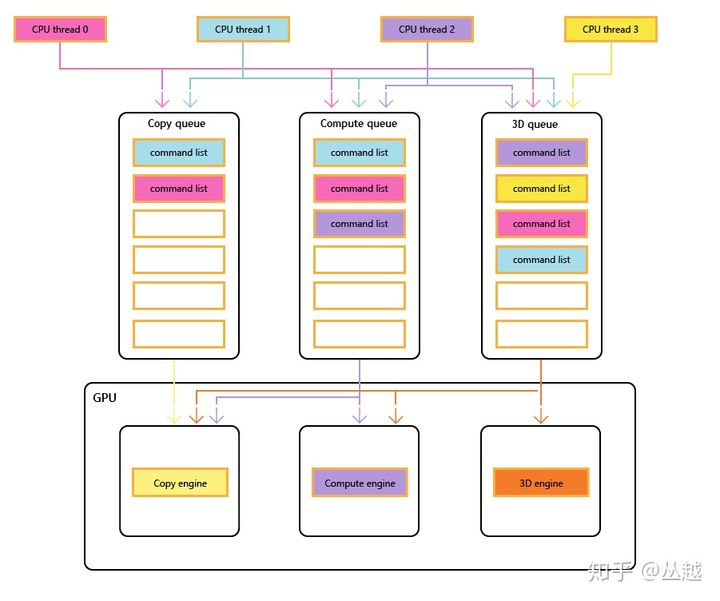
\includegraphics[width=10cm]{rendering_framework.jpg}
  \centering
  \caption{GPU硬件功能抽象}
  \label{fig:gpu_hardware_abstraction}
\end{figure}

利用这个机制可以将管线设计为这样:
\begin{figure}[H]
  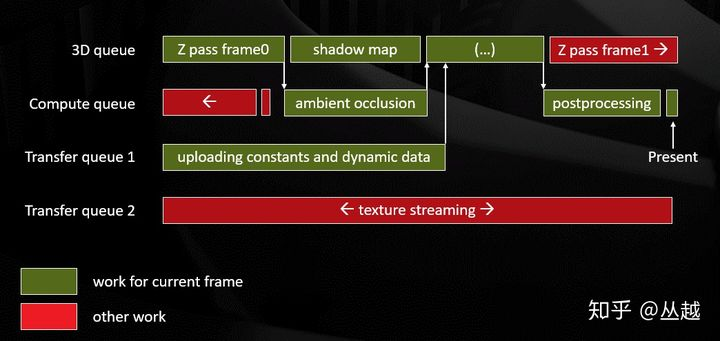
\includegraphics[width=10cm]{rendering_pipeline_design.jpg}
  \centering
  \caption{GPU渲染管线的初步设计}
  \label{fig:gpu_rendering_pipeline_design_0}
\end{figure}

如图所示, 图形(3D)队列负责 PreZ、GBuffer、Shadow 等场景渲染, 同时计算队列负责计算后处理(SSAO、Bloom、ToneMapping、AA 等等), Copy 队列同时执行纹理 Streaming 或者 Virtual texture 等操作。这些都可以在 GPU 时间线上同时进行, 大大提高了渲染管线的性能.

进一步优化 Render Graph:
通过检查渲染帧内的资源依赖关系, 利用别名资源重复利用内存堆, 优化 GPU 内存资源使用。如下所示:

\begin{figure}[H]
  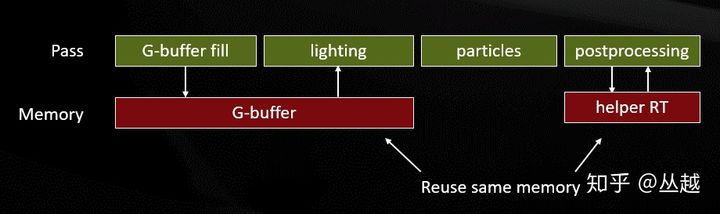
\includegraphics[width=10cm]{rendering_pipeline_design_opt.jpg}
  \centering
  \caption{GPU渲染管线进一步优化}
  \label{fig:gpu_rendering_pipeline_optimization}
\end{figure}

GPU驱动的渲染管线
利用间接绘制/计算(IndirectDraw/IndirectCompute), 可实现渲染时更少的CPU/GPU之间的切换, 在CPU中准备场景数据, 一次性提交到GPU中, 使用GPU进行可见性剔除, 并填充CommandList/Buffer, 这样可以将传统的CPU负担的工作交由GPU执行, 降低CPU的负载, 甚至可以进行更高精度级别的可见性剔除.
\begin{figure}[H]
  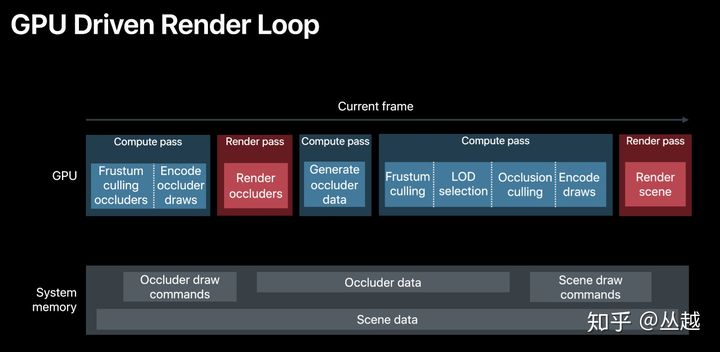
\includegraphics[width=10cm]{gpu_driven_rendering.jpg}
  \centering
  \caption{基于Metal API的GPU驱动渲染管线设计}
  \label{fig:gpu_rendering_pipeline_optimization}
\end{figure}

\section{深入GPU硬件运行机制\cite{deepIntoGPU}}
\subsection{GPU中的几个基本概念}
这里以Nvidia Turing架构为例, Turing架构是Nvidia在2018年发布的GPU架构, 其下2060、2080系列显卡均使用该种架构.
\begin{figure}[H]
  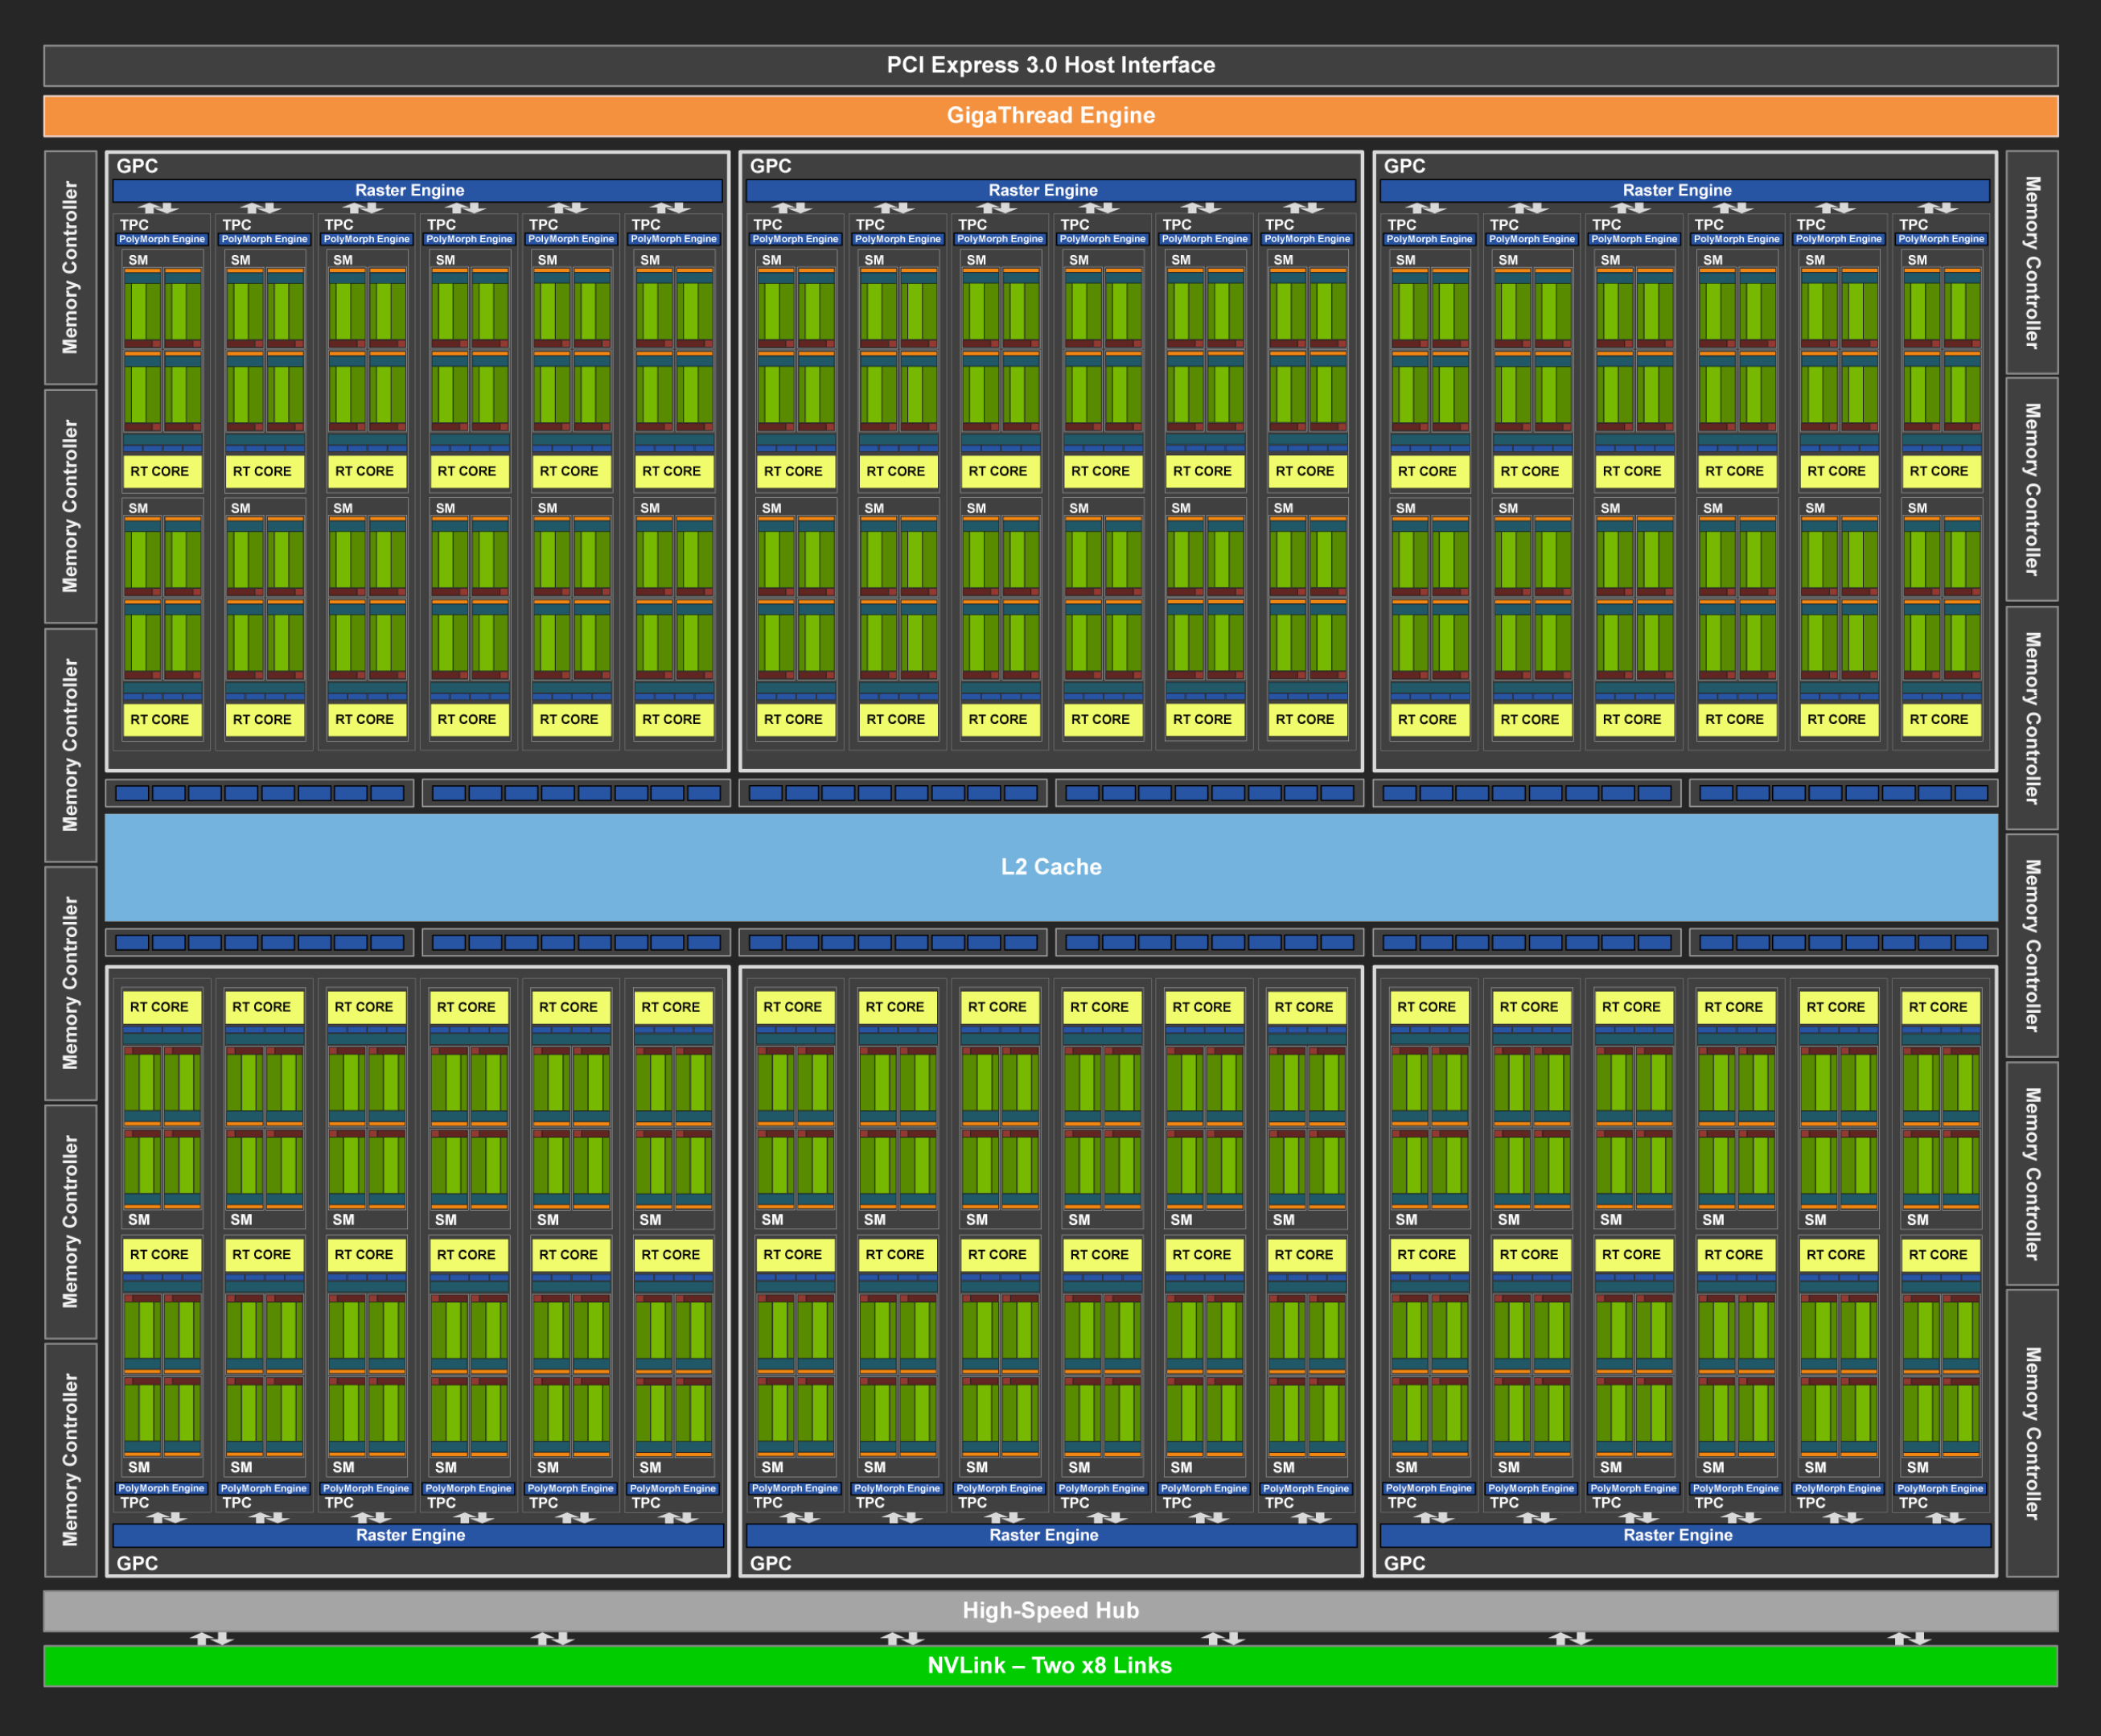
\includegraphics[width=18cm]{nvidia_turing.png}
  \centering
  \caption{Nvidia Turing架构}
  \label{fig:nvidia_turing}
\end{figure}

\begin{figure}[H]
  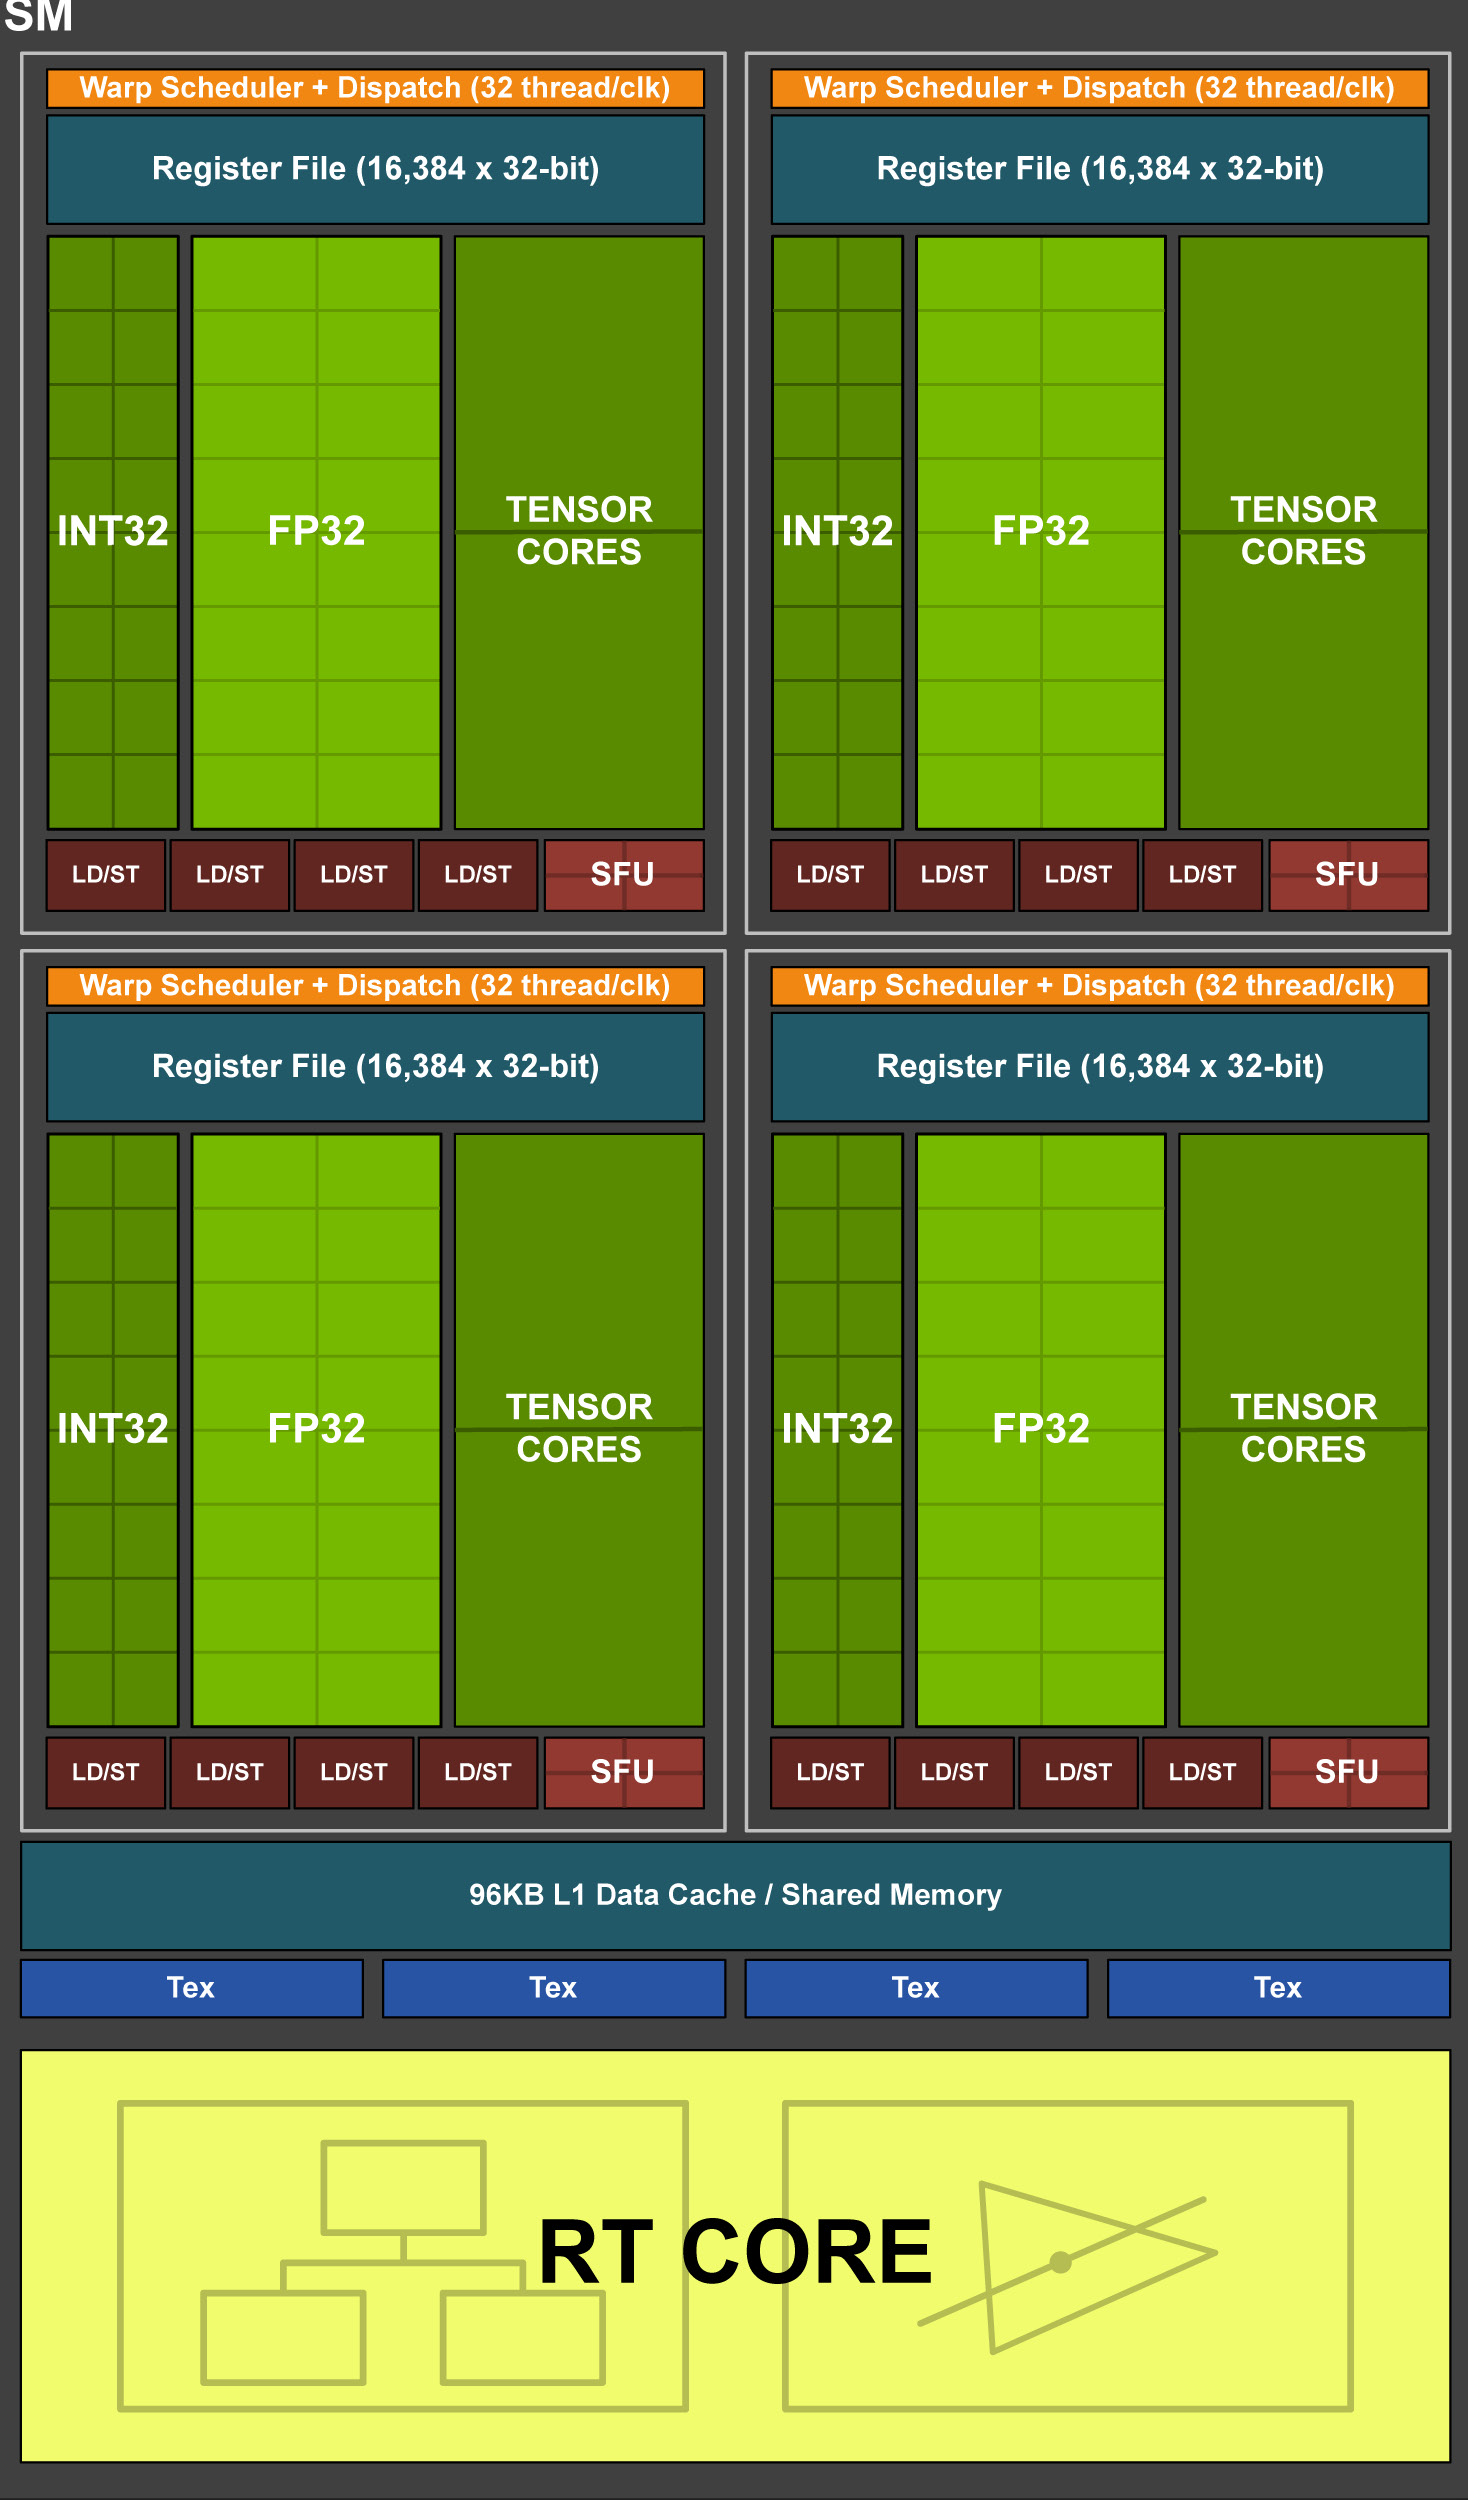
\includegraphics[width=10cm]{nvidia_turing1.png}
  \centering
  \caption{Nvidia Turing架构-Stream Multiprocessor}
  \label{fig:nvidia_turing_SM}
\end{figure}

GPU中的一些基本概念如下:
\begin{itemize}
\item Giga Thread Engine
  管理所有正在进行的工作
\item GPC(Graphics Processing Cluster)
  \\GPU被划分成多个GPCs(Graphics Processing Cluster),每个GPC拥有多个SM(SMX、SMM)和一个光栅化引擎(Raster Engine).
  \begin{itemize}
  \item Raster Engine
  \item TPC(Texture Processing Cluster)
    \begin{itemize}
    \item PolyMorph Engine
      \\多边形引擎负责属性装配(attribute Setup)、顶点拉取(VertexFetch)、曲面细分、栅格化(这个模块可以理解专门处理顶点相关的东西)
    \item Register File
    \item SM(Stream Multiprocessor)
      \\多个sp加上其他的一些资源组成一个SM, 其他资源也就是存储资源, 共享内存, 寄储器等.
    \item Warp(Warp Schedular+Dispatch)
      \\多个SP(一般是32个)组成一个Warp, Warp是最小调度单位. 同一个Warp内的SP执行指令相同只是数据不同. 只有全部线程执行完毕才会进行下一个Warp的工作.
    \item SP(Stream Processor)/Core/Thread
      \\SP是最基本的处理/计算单元.
      \begin{itemize}
      \item ALU
      \item FPU
      \item Tensor Core
      \end{itemize}
    \item SFU
      \\特殊数学函数, 如sin, cos, 与普通sin, cos实现(一般会查表)不同.
    \item L1 Cache
    \item Texture Cache
    \item LD/ST
    \item RT(RayTracying) Core
    \end{itemize}
  \end{itemize}
\item Grid
  \\编程中的一个概念. 指在GPU上由多个Thread block(SM)执行的一套代码.
\end{itemize}

GPU的内存可以分为四级:
\begin{center}
  \begin{tabular}{|c c c c|} 
    \hline
    More descriptive name & Closest old term outside of GPUs & Official Nvidia GPU term & Description \\ [0.5ex] 
    \hline\hline
    GPU Memory & Main Memory & Global Memory & DRAM memory accessible by all multithreaded SIMD Processors in a GPU.\\
    \hline
    Private Memory & Stack or Thread Local Storage (OS) & Local Memory & Portion of DRAM memory private to each SIMD Lane.\\
    \hline
    Local Memory & Local Memory & Shared Memory & ast local SRAM for one multithreaded SIMD Processor, unavailable to other SIMD Processors\\
    \hline
    \\SIMD Lane Registers & Vector Lane Registers & Thread Processor Registers & Registers in a single SIMD Lane allocated across a full thread block (body of vectorized loop).\\
    \hline
  \end{tabular}
\end{center}







\bibliography{bibliography.bib}
\end{document}
